\documentclass[11pt,a5paper]{article}

\usepackage[T1]{fontenc} % font encoding, lubab õ tähte kasutada
\usepackage[utf8]{inputenc} % oleme siiski 21. sajandis, vajadusel on ka olemas utf8x
\usepackage{lmodern} % lmodern ja micrtype käivad käsikäes, teeb teksti ilusamaks
\usepackage{microtype}
\usepackage[estonian]{babel} % eesti keele poolitamisreeglid jpm
\usepackage[per = fraction, expproduct=cdot, decimalsymbol=comma, inter-unit-product=\cdot]{siunitx} % http://www.bakoma-tex.com/doc/latex/siunitx/siunitx.pdf
\usepackage{graphicx}
\usepackage{wrapfig}
\usepackage{tikz}
\usepackage[european]{circuitikz}
\tikzset{component/.style={draw,thick,circle,fill=white,minimum size =0.75cm,inner sep=0pt}}
\usepackage{amsmath,amssymb}
\usepackage{amsfonts}
\usepackage{epstopdf} %minul on vaja, et .eps pilte saada
\usepackage{enumitem}
%paneme kõik mõõdud paika
\topmargin=-3.0cm \textheight=19cm \textwidth=12.9cm
\oddsidemargin=-1.5cm  \evensidemargin=-1.5cm
\setlength{\parindent}{0pt} \setlength{\parskip}{6pt} \sloppy
\relpenalty=10000 \binoppenalty=10000 % Tekstisisestes valemites reavahetusi ärgu olgu
\pagestyle{empty} % ilma leheküljenumbrita
\newcommand{\numb}[1]{\vspace{5pt}\textbf{\large #1}}
\newcommand{\nimi}[1]{(\textsl{\small #1})}
\newcommand{\punktid}[1]{(\emph{#1~p.})}
\newcounter{ylesanne}
\newcommand{\yl}[1]{\addtocounter{ylesanne}{1}\numb{\theylesanne.} \nimi{#1} \newblock{}}
\newcommand{\autor}[1]{\emph{ Autor: #1.\\}}
\newcommand{\lautor}[1]{\emph{ Lahenduse autor: #1.\\}}


\begin{document}

\begin{center}
\textbf{\Large Eesti koolinoorte 67. füüsikaolümpiaad} \vspace{2pt}

\emph{9. juuni 2020. a. Lõppvoor.}

\emph{{\bf Gümnaasiumi} ülesannete lahendused}

\end{center}

\yl{KLAASKERA}
\punktid{6}
\autor{Hans Daniel Kaimre}
Mööda optilist peatelge liikuv kiir ei murdu ning liigub otse läbi kera. Seega koonduvad kõik kiired kera tagumise poole ja optilise peatelje lõikumiskohta. Uurime nüüd üht valguskiirt, mis asub vihu tsentrist eemal. Selle konkreetse valguskiire jaoks võib lähendada probleemi kahedimensionaalseks. Joonistame kiire käigu, märgime nurgad. Langemisnurk olgu $\alpha$ ning murdumisnurk $\beta$, kusjuures need on omavahel seotud Snelli seadusega: $n_{õ}\sin\alpha=n_{k}\sin\beta$. Sarnaste kolmnurkade tõttu $\angle AOB$ on samuti $\alpha$. Kolmnurk $AFO$ on võrdhaarne (haaradeks kera raadiused) ning seega $\angle AFO$ on $\beta$. Ühelt poolt (kolmnurga sisenurkade summa on $180^\circ$) $\angle AOF=180-2\beta$, teisalt (kõrvunurkade summa on $180^\circ$) $\angle AOF=180^\circ-\alpha$, seega $\alpha=2\beta$. Võttes, et $n_{õ}=1$ ning tehes väikeste nurkade lähenduse $\sin x \approx x$, saame:
$$n_{õ}\sin\alpha=n_{k}\sin\beta \Rightarrow \sin2\beta=n_{k}\sin\beta \Rightarrow n_k = \frac{\sin2\beta}{\sin\beta}\approx\frac{2\beta}{\beta}=2.$$
\begin{figure}[htbp!]
\centering
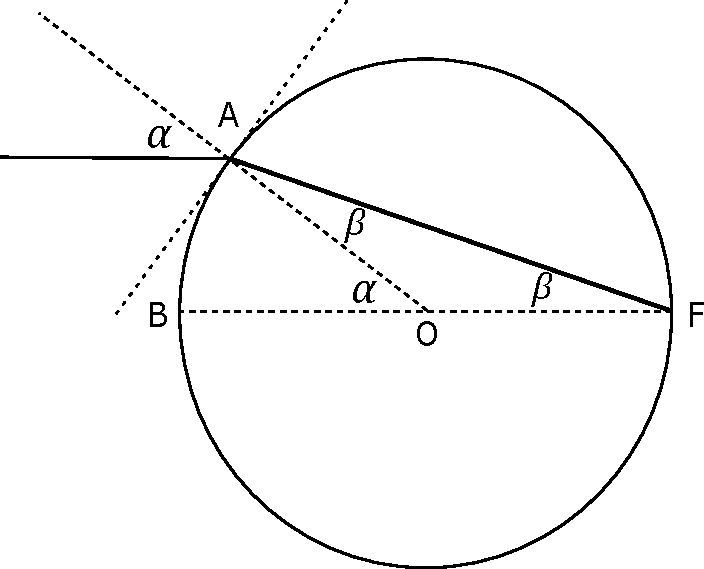
\includegraphics[width=0.6\textwidth]{klaasistkera_joonis.pdf}
\end{figure}

\yl{KOHUKESED}
\punktid{8}
\autor{Kaarel Hänni}
Koti mõõtmed on Richardi käe pikkusega võrreldes väikesed, seega võime eeldada, et nurkkiirendus on kõigile kohukestele ühtemoodi $\omega^2 \ell$, kus $\ell$ on Richardi käe pikkus. Kohukesed ei kuku kotist välja, seega ringi ülemisest punktist saame $\omega^2\ell\geq g$. Kohukesed ei lähe alumises punktis lömaks, seega rõhk $\rho (g+\omega^2 \ell) h$ pole piisav, et kohukest lömastada. Eelnevast
\[\rho (g+\omega^2 \ell) h\geq \rho g 2h.\]

Seega saaks kotti panna kõrgusega $2h$ kihi kohukesi, ilma et need lömaks läheks.

\yl{KÄIVITUSVOOL}
\punktid{8}
\autor{Valter Kiisk}
Vasktoru takistus on ilmselt märksa väiksem kui ampermeetri sisetakistus, seega praktiliselt kogu käivitusvool kulgeb läbi vasktoru.

Vasktoru ristlõike pindala (mida vool läbib) on $S=\frac{1}{4}\pi(d_2^2-d_1^2)=\SI{22}{\milli\meter\squared}$. Ühikulise pikkusega torujupi takistus on $R=\rho/S$. Seega voolutugevusel $I_1=\SI{500}{A}$ pingelang vasktoru pikkusühiku kohta
\[
\delta U = RI_1 = \frac{\rho}{S}I_1\approx \SI{0.38}{\volt\per\meter}.
\]
Et läbi ampermeetri tekiks voolutugevus $I_0=\SI{1}{mA}$, on ampermeetrile tarvis rakendada pinge $U=I_0R_0=\SI{0.1}{\volt}$. Selline pingelang moodustub vasktoru pikkusel $\ell=U/\delta U=\SI{0.26}{\meter}$.

\yl{TASAKAALULIIKUR}
\punktid{8}
\autor{Krister Kasemaa}
Hannese liikumist saab vertikaalsuunas käsitleda vedrupendli võnkumisena. Vedrupendli perioodi valem on: $$T=2\pi \sqrt{\frac{m}{k}}$$ Kuna meie süsteemil on kaks vedru rööbiti, tuleb võngete perioodi valemit veidi muuta. Kahe kõrvuti oleva vedru jäikus on võrdne ühe vedruga, mille jäikus on eelnevate vedurude jäikuste summaga. Seega on meie süsteemi vertikaalsuunaliste võngete periood:
$$T = 2\pi \sqrt{\frac{m}{2k}}$$
Resonants tekib, kui koosinuslaine läbimise sagedus ühtib verikaalse vedrusüsteemi naturaalsagedusega. Seega peab Hannes $\Delta x = \SI{6}{m}$ võrra edasi liikuma sama ajaga, mil teeb masspendel ühe naturaalsagedusel võnke. Seega, resonantsi tekke kiirus:
$$v_\mathrm{resonants}=\frac{\Delta x}{T}=\frac{\Delta x}{2 \pi} \sqrt{\frac{2k}{m}} = \SI{4.678}{m s^{-1}} \approx \SI{4.7}{m s^{-1}}$$

\yl{GLOOBUS}
\punktid{10}
\autor{Rael Kalda}
\osa Pöördsümmeetria tõttu on näha, et väljundklemmide \emph{A} ja \emph{C} vahele jäävatel sõlmedel on kõigil sama potentsiaal. Seega võib need neli sõlme kokku ühendada ja saame kaks järjestikust neljatakistilist rööbitiühendust:\\
\begin{center}
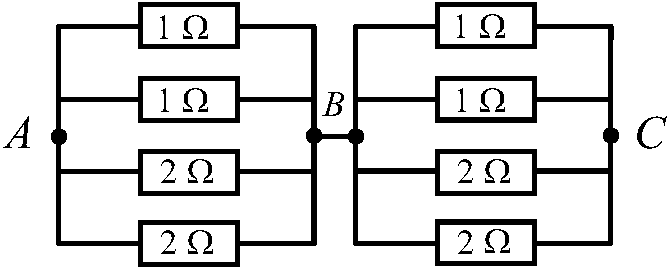
\includegraphics[scale=0.8]{gloobus0.pdf}\\
\end{center}
Takistus \emph{A} ja \emph{C} vahel on seega: $$2 \cdot \frac{1}{\displaystyle{2 \cdot \frac{1}{2} + 2 \cdot \frac{1}{1}}} \,\, \SI{}\Omega=\frac{2}{3} \, \SI{}\Omega.$$

\osa \emph{Variant 1:} Kerast on võimalik saada ekvivalentne skeem:\\
\begin{center}
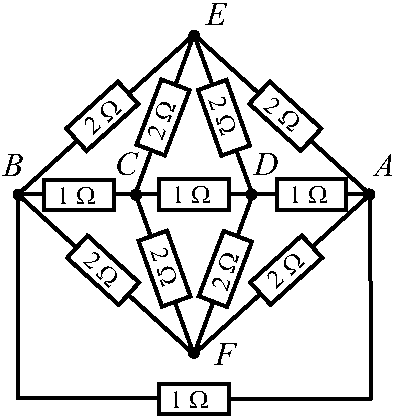
\includegraphics[scale=0.8]{gloobus1.pdf}\\
\end{center}
kus on lisatud veel sõlmede tähised \emph{D}, \emph{E} ja \emph{F}. Kuna sõlmedel \emph{E} ja \emph{F} on sama potentsiaal, saame need kokku ühendada sõlmeks \emph{O}, nagu järgneval skeemil. Sel juhul on sõlmega \emph{O} ühendatud neli takisti paari, kus üks paar, mis koosneb kahest rööbiti ühendatud 2-oomisest takistist, annab kokku tavalise 1-oomise takisti:
\begin{center}
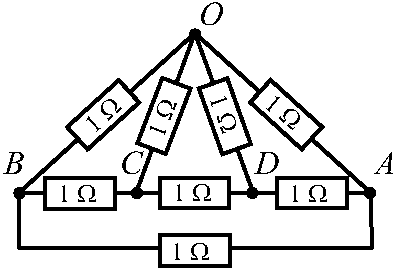
\includegraphics[scale=0.8]{gloobus2.pdf}\\
\end{center}
Nüüd saame tänu sümmeetriale sõlme \emph{O} poolitada:
\begin{center}
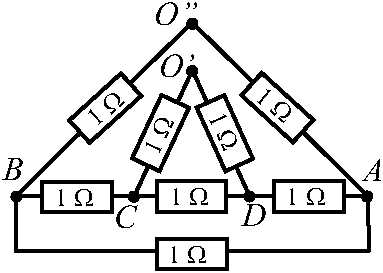
\includegraphics[scale=0.8]{gloobus3.pdf}\\
\end{center}
Uue skeemi järgi arvutame \emph{A} ja \emph{B} vahelise takistuse:

$$ \frac{1}{\frac{1}{\displaystyle{\frac{1}{\frac{1}{2}+1} + 1 \cdot 2}}+\frac{1}{2}  + 1} \,\, \SI{}\Omega =\frac{8}{15} \, \SI{}\Omega.$$

\emph{Variant 2:} Muutes \emph{C} ja \emph{D} vahelise takistise kaheks 0,5-oomiseks jadamisi takistiks ja öeldes, et \emph{C} ja \emph{D} keskel on uus punkt \emph{O}, siis on \emph{E},\emph{F} ja \emph{O} sama pingega ning need saab ühendada üheks punktiks. Sellega taandub skeem jadamisi ja rööbiti ühendusteks:
\begin{center}
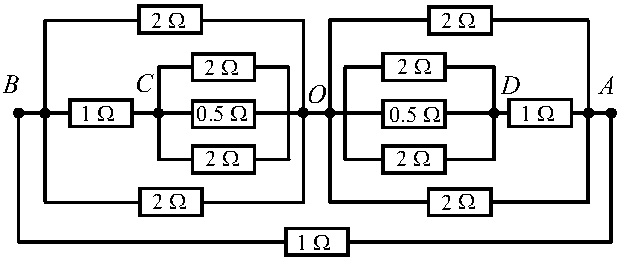
\includegraphics[scale=0.9]{gloobus4.pdf}\\
\end{center}
mille kogutakistuse välja arvutamisel saame samuti $\frac{8}{15} \, \SI{}\Omega$.


\yl{PALLIVISKENÕLV}
\punktid{10}
\autor{Kaarel Hänni}
%Allikas -- \url{https://www.usna.edu/Users/physics/mungan/_files/documents/Scholarship/Projectile.pdf}
\emph{Lahendus 1.}
Ilmselgelt viskab Oleg kaugeimale, kui ta viskab oma maksimaalse kiirusega $v$, mis ei sõltu viskesuunast. Olgu viskenurk horisontaalsihi suhtes $\theta$. Kõrguselt $h$ visates saame liikumise vertikaalsest komponendist lennuaja $t$ jaoks järgmise võrrandi:
\[h=\frac{gt^2}{2}-t\sin \theta v.\]
Horisontaalsuunas liikumisest saame viske pikkusest $\ell$ avaldada aja:
\[t=\frac{\ell}{v\cos \theta}.\]

Asendades selle sisse esimesse võrrandisse, saame
\begin{equation}\label{main}
    h(1+\cos 2\theta)=\frac{g\ell^2}{v^2}-\ell\sin 2\theta.
\end{equation}

Fikseerides $h$, me otsime $\ell=\ell(\theta)$ maksimumi. Maksimumi leidmiseks võtame ülemise võrrandi mõlemast poolest tuletise $\theta$ järgi ja kasutame ära, et maksimumis $\frac{d\ell}{d\theta}=0$, saades
\[\tan 2\theta=\frac{\ell}{h},\]
millest
\[cos2\theta=\frac{h}{\sqrt{h^2+\ell^2}}, \sin 2\theta=\frac{\ell}{\sqrt{h^2+\ell^2}}.\]

Asendades need sisse võrrandisse \ref{main}, saame

\[\ell=\frac{2v^2}{g}\left(h+\frac{v^2}{2g}\right).\]

$h=0$ juhust saame
\[L=\frac{v^2}{g}.\]

Asendades selle sisse avaldisse $\ell$ jaoks, saame
\[\ell=L\sqrt{1+2\frac{h}{L}}.\]

Seega peab nõlva kõrgusel $y=h$ olev punkt olema keskjoonest kaugusel $L\sqrt{1+2\frac{h}{L}}$. Seega keskjoone suhtes on nõlva võrrand
\[x=L\sqrt{1+2\frac{y}{L}}.\]

Nihutades $x$-koordinaadi $0$-punkti väljaku otsajoone juurde, saame
\[x=L\left(\sqrt{1+2\frac{y}{L}}-1\right).\]

\emph{Lahendus 2.}
\emph{Jaan Kalda}
Vaatleme suvalist viskamispunkti nõlval ja kasutame seda $\xi-\eta$~koordinaadistiku nullpunktina. Teatavasti on punktist $(0;0)$ kiirusega $v$ visates tabatava ruumipiirkonna piirjoon $\eta=\frac{v^2}{2g}-\frac{g\xi^2}{2v^2}$. See on parabool, mille tipp on kõrgusel $\frac{v^2}{2g}$ viskepunkti kohal. On ilmne, et väljaku keskpunkt lebab sellel joonel. Peegeldame seda parabooli horisontaaltasandi suhtes ja nihutame nii, et uue parabooli tipp oleks $\frac{v^2}{2g}$ sügavusel väljaku keskpunkti all: $y=-\frac{v^2}{2g}+\frac{gx^2}{2v^2}$, kus  $x-y$~koordinaadistiku nullpunkt on väljaku keskpunkt. Sümmeetria tõttu lebab viskamispunkt sellel uuel kõveral. Uue parabooli kuju ei sõltu viskamispunkti asukohast, seega asuvad kõik viskamispunktid sellel paraboolil.

Soovi korral võime valemi esitada kasutades väljaku poolpikkust $L=v^2/g$: $y=-\frac L2+\frac{x^2}{2L}$. Samuti võime nullpunkti nihutada väljaku serva, $y=x'(x'-2L)/2L$.


\yl{PULGAD}
\punktid{12}
\autor{Richard Luhtaru}
\osa Olgu silindrile mõjuv normaaljõud kummaski punktis $N$ (puutujaga risti) ning hõõrdejõud $F_h$ (puutujaga paralleelne). Olgu nurk pulkade vahel $2\alpha$.

\begin{figure}[h]
\centering
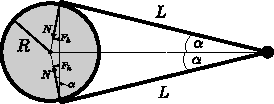
\includegraphics[width=0.5\linewidth]{pulgad_lah_joon.pdf}
\end{figure}

Jõudude tasakaalust saame, et puutepunktides mõjuvad resultantjõud $\vec N + \vec{F_h}$ peavad olema paralleelsed ja vastassuunalised, seega sümmeetria tõttu peab $\vec N + \vec{F_h}$ olema sümmeetriateljega risti.

Kuna puutuja on raadiusega risti, on lihtne näidata, et nurk $\vec N$ ja puutepunkte ühendava sirge vahel on $\alpha$, seega $\tan \alpha = \frac{F_h}{N}$. Piirjuhul, kus $\mu$ on minimaalne, $F_h = \mu N$ ja seega
$$\tan \alpha = \frac{\mu N}{N} = \mu$$

Teisalt $\tan \alpha = \frac{R}{L}$, seega
$$\mu_\text{min} = \frac{R}{L}$$

\osa Nagu eelmises osas näidatud, siis hõõrdejõu lauaga paralleelne komponent $F_{h,r} = N\tan \alpha = \frac{R}{L}\cdot N$. Silindrit üles tõstes peab raskusjõu tasakaalustamiseks lisaks mõjuma kummaski punktis hõõrdejõu lauaga risti olev komponent $F_{h,t} = \frac{mg}{2}$, seega kui summaarne hõõrdejõud on $F_h$, siis
$$F_h^2 = F_{h,r}^2 + F_{h,t}^2 = \frac{R^2}{L^2}N^2 + \frac{m^2g^2}{4}$$

Piirjuhul $F_h = \mu N$ ja $\tau = NL$, seega
$$\mu^2N^2 = \frac{R^2}{L^2}N^2 + \frac{m^2g^2}{4}$$
$$\left(\mu^2 - \frac{R^2}{L^2}\right)N^2 = \frac{m^2g^2}{4}$$
$$N = \frac{mg}{2\sqrt{\mu^2-\frac{R^2}{L^2}}}$$
$$\tau_\text{min} = NL = \frac{mgL}{2\sqrt{\mu^2-\frac{R^2}{L^2}}} = \frac{mgL^2}{2\sqrt{L^2\mu^2 - R^2}}$$

\yl{OPTILINE SEADE}
\punktid{12}
\autor{Jaan Kalda}
\begin{figure}[h]
\centering
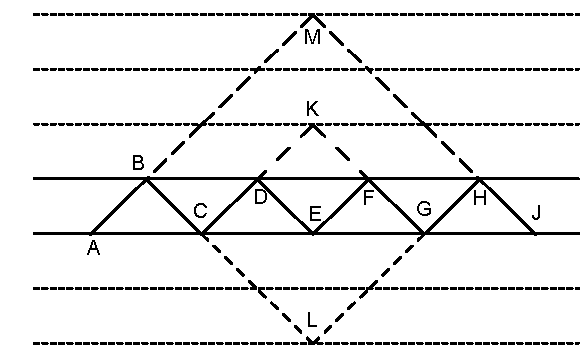
\includegraphics[width=0.5\linewidth]{optiline-silinder-lah1.pdf}\par
Joonis 1
\end{figure}
Kõigepealt vaatleme kiirte käiku kahe paralleelse peegli vahel joonisel 1. Kui peegeldame sik-sakilisest kiirest jupi $DEF$ ülemises peeglis, saame jupi $DKF$, mis koos lõikudega $CD$ ning $FG$ moodustab juba vähemate sik-sakkidega jupi $CKG$. Peegeldades juppi $CKG$  alumises peeglis saame jupi $CLG$ ning korrates peegeldamist veel ühe korra saame tervest sik-sakilisest teekonnast $ABCDEFGHJ$ teekonna $AMJ$, mida võib vaadelda kui kiire $AB$ peegeldust alumise peegli kujutise-kujutise-kujutises. Niisiis, kui joonistame peeglite kujutised, kujutise-kujutised jne, näeme, et sisenevad kiired justkui peegelduksid peeglite kujutises või kujutise-kujutises või kujutise-kujutise-kujutises jne. Algsel joonisel toodud kiirte põhjal saame taastada kaks sellist kujutist, kujutise-kujutist või kujutise-kujutise-kujutist  või jne. N-järku kujutiste seeria moodustab paralleelsete sirgete rivi; tegelikud peeglid peavad olema ühed neist. Kui me joonistame sisendkiiri väljundkiirteks peegeldavate  sirgetega (mis on leitavad kiirte pikenduste lõikepunkte läbivate nurgapoolitajate ristsirgetena) paraleelsete ja võrdsetel vahekaugustel asuvate sirgete rivi, siis peavad tegelikud peeglid asuma kahel naabersirgel.

\begin{figure}[h]
\centering
  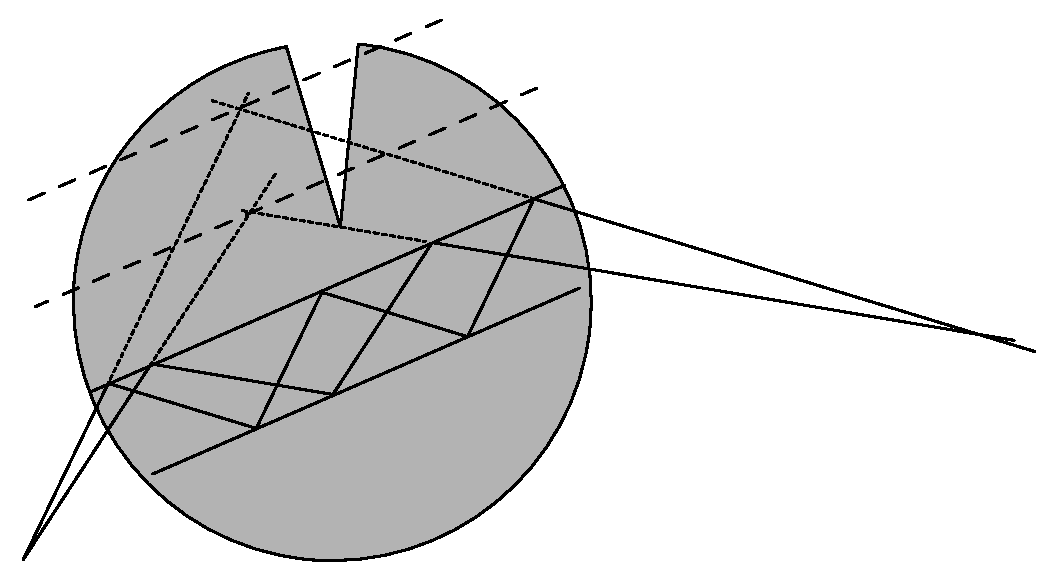
\includegraphics[width=0.4\textwidth]{optiline-silinder-lah2.pdf}
  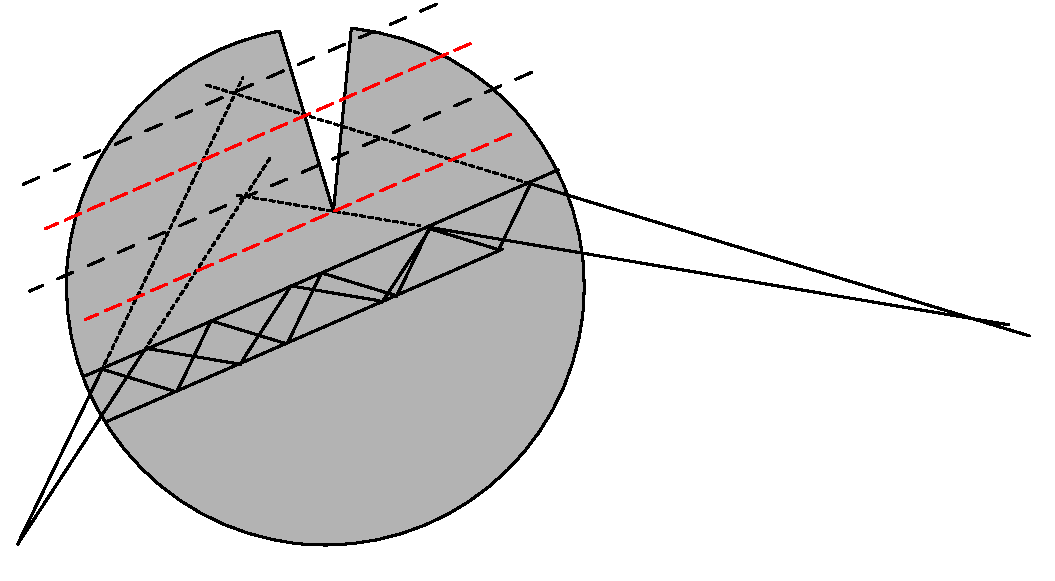
\includegraphics[width=0.4\textwidth]{optiline-silinder-lah3.pdf}
  \par
  \begin{tabular}{p{0.5\linewidth}p{0.5\linewidth}}
  \hfil Joonis 2. & \hfil Joonis 3. \\
  \end{tabular}
\end{figure}

Joonisel 2 on näha, et lihtsaimal juhul välistab sisselõige peeglite asukoha kõigis peale kahe alumise (veel madalamad asukohad pole võimalikud seetõttu, et sisendkiired ei saa nende vahele siseneda). Põhimõtteliselt on võimalik ka joonisel 3 toodud variant.

\yl{ÕHUPALLID}
\punktid{12}
\autor{Taavet Kalda}
Õhupallide raadiuste erinevus on põhjustatud õhupalli kasutatavate materjalide erinevusest. Gaasi rõhku tasakaalustab õhupallide materjali venivusest tulenev pinge. Jõudude tasakaalu arvutamiseks vaatleme õhupalli ristlõiget mis jagab õhupalli kaheks võrdseks pooleks. Kuna mõlemad pooled on tasakaalus, peab õhu avaldatud rõhumisjõud ühele õhupalli poolele tasakaalustama õhupalli sisemised jõud. Olgu õhupalli raadius $r$, ruumala $V$, materjali paksus $\delta r$, Youngi moodul $E$, õhu rõhk õhupalli sees $p$ ning materjali pinge $\sigma$. Siis jõudude tasakaal esitub kujul
\[
\pi r^2 p = 2\pi r\delta r \sigma,
\]
kus me eeldasime et $r \gg \delta r$. Õhupalli deformatsioon on ligikaudu $\epsilon = r / r_0$, kus $r_0$ on õhupalli esialgne karakteerne lineaarmõõde. Seega, $\sigma = Er/r_0$. Lisaks kehtib õhupalli materjali massi (ehk ruumala) jäävus. Teisisõnu, $r^2\delta r = \alpha$, kus $\alpha$ on konstant. Kokkuvõttes saame, et
\begin{equation}
p = \frac{1}{\pi r^2} \frac{2\pi r^2\delta rE}{r_0} = \frac{2\alpha E}{r_0}\frac{1}{r^2}  = k/r^2,
\label{ohupall-1}
\end{equation}
kus $k = 2\alpha E/r_0$ on õhupallile omane konstant. Ideaalse gaasi olekuvõrrandist saame
\[
n = \frac{pV}{RT} = \frac{4\pi}{3RT}pr^3 = \frac{4\pi k}{3RT}r.
\]
Või siis
\[
n = Akr,
\]
kus $A$ on kõikidele õhupallidele ühine konstant. Niisiis, kuna mõlemas õhupallis on sama palju õhku, siis
\begin{equation}
k_1r_1 = k_2r_2.
\label{ohupall-2}
\end{equation}
Edasi, ühendades õhupallid toruga, hakkab õhk suurema rõhuga õhupallist voolama teise õhupalli. Samas paneme tähele, et õhupalli rõhk on pöördvõrdeline raadiuse ruuduga. See tähendab, et mida väiksemaks õhupall muutub, seda kiiremini see tühjenema hakkab, sest õhurõhk aina suureneb. Seega tühjeneb esialgselt suurema rõhuga õhupall täielikult. Ülesande eelduste kohaselt ei pea tühjeneva õhupali deformatsioonivaba mõõtmetega arvestama.

Kombineerides võrrandid (\ref{ohupall-1}) ja (\ref{ohupall-2}) näeme, et
\[
\frac{p_1}{p_2} = \frac{k_1}{k_2} \frac{r_2^2}{r_1^2} = \frac{r_2^3}{r_1^3}.
\]
Kuna $r_1 > r_2$, siis teine õhupall hakkab kiiremini tühjenema ning seega, $R_2 = 0$. Esimeses õhupallis on $2n$ molekuli, st
\[
2n = Ak_1 R_1 = \frac{n}{r_1}R_2.
\]
Seega,
\[
R_1 = 2r_1.
\]

\yl{RUUT}
\punktid{14}
\autor{Kaur Aare Saar}
Olgu $M$ ja $N$ vastavalt $AB$ ja $CD$ keskpunktid. Superpositsioneerime
ruudu, kus pinge on rakendatud $A$ ja $C$ vahele, ruuduga, kus pinge on
rakendatud $B$ ja $D$ vahele. Nüüd sümmeetria tõttu telge $MN$ ei läbi vool
ehk takistus $A$ ja $D$ vahel ristkülikus $AMND$ on samuti $R$. Peegeldame
$MN$ üle $AD$. Saame ruudu $M'MNN'$, külgede keskpunktidega $A$ ja $D$. $A$ ja
$D$ vaheline takistus sellises ruudus on kaks korda väiksem ehk $R/2$.

\end{document}
